\documentclass[tikz]{standalone}


\usepackage{tikz}
\usetikzlibrary{calc}

\begin{document}
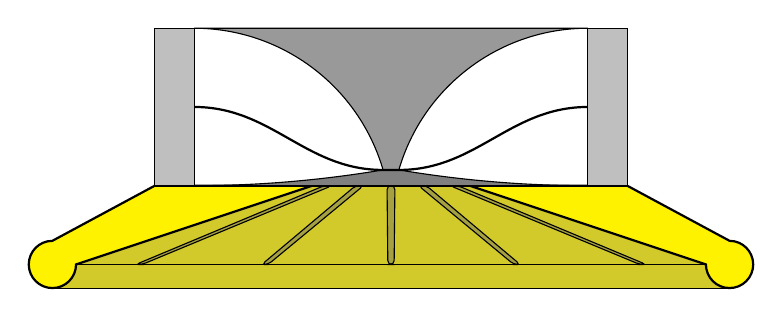
\begin{tikzpicture}[
	scale=1,
	membran/.style={thick},
	DEA1/.style={draw, fill=gray},
	DEA2/.style={draw, fill=gray!80},
	housing/.style={draw, fill=gray!50}
]




%%% SUCKER


\path
(-1, 1)coordinate(1L)--(-4,0)coordinate(2L)arc(0:-270:.3)--(-2.5,1.5)--(2.5,1.5)--(4.3,.3)arc(90:-180:.3)coordinate(2R)--(1,1)coordinate(1R) 
;
\fill[yellow!80!black](1L)--(1R)--(2R)--++(.3,-.3)--($(2L)+(-.3,-.3)$)--(2L);
\draw (1L) -- (1R);
\draw (2L) -- (2R);
\draw[] (2L)++(-.3,-.3)--($(2R)+(.3,-.3)$);

\foreach \pos in {.1,.3, .5, .7, .9}{
	\path (1L)--(1R)coordinate[pos=\pos-.025](11);
	\path (1L)--(1R)coordinate[pos=\pos+.025](12);
	\path (2L)--(2R)coordinate[pos=\pos-.005](21);
	\path (2L)--(2R)coordinate[pos=\pos+.005](22);

	\draw[fill=yellow!60!black,
	rounded corners = .5mm	
	] (11)--(21)--(22)--(12)--cycle; %  node{2};
}


\draw[
	thick,
	fill=yellow,] 
(-1, 1)coordinate(1L)--(-4,0)coordinate(2L)arc(0:-270:.3)--(-3,1)--(3,1)--(4.3,.3)arc(90:-180:.3)coordinate(2R)--(1,1)coordinate(1R) 
;




%%% DEA Mechansim
\begin{scope}[yshift=1cm]
\def\h{2}	% height
\def\b{2.4}
\def\db{.1} % total width = 2*(\b+\db+\bh)
\def\bh{.5} % housing width
\def\x{.1}  % between 0.01 and .99 .. relative height

\pgfmathsetmacro{\Ri}{\b^2/(2*\h*\x) + \h*\x/2}
\pgfmathsetmacro{\Rii}{\b^2/(2*\h*(1-\x)) + \h*(1-\x)/2}
\pgfmathsetmacro{\alpi}{asin(\b/\Ri)}
\pgfmathsetmacro{\alpii}{asin(\b/\Rii)}


\path[DEA1] (-\b-\db,0)arc(-90:-90+\alpi:\Ri)--++(2*\db,0)arc(270-\alpi:270:\Ri)--cycle;
\path[DEA2] (-\b-\db,\h)arc(90:90-\alpii:\Rii)--++(2*\db,0)arc(-90+\alpii:-90:-\Rii)--cycle;

\draw[membran] (-\b-\db,\h*.5) to[out=0, in=180](-\db,\h*\x)--++(2*\db,0)to[out=0, in=180](\b+\db,\h*.5);

\path[housing] (-\b-\db,0)rectangle++(-\bh,\h);
\path[housing] (+\b+\db,0)rectangle++(\bh,\h);
\end{scope}


\end{tikzpicture}
\end{document}